
  \section{Deep Learning Model}
  
  The Features formed from data processing block are then subjected to deep learning model. The implementation is done using  using keras library in python. The implemented model is represented by Figure ~\ref{fig:dlm}. The input layers are described in table ~\ref{table:inputs}.
  
  \begin{figure}[H]
  \centering
  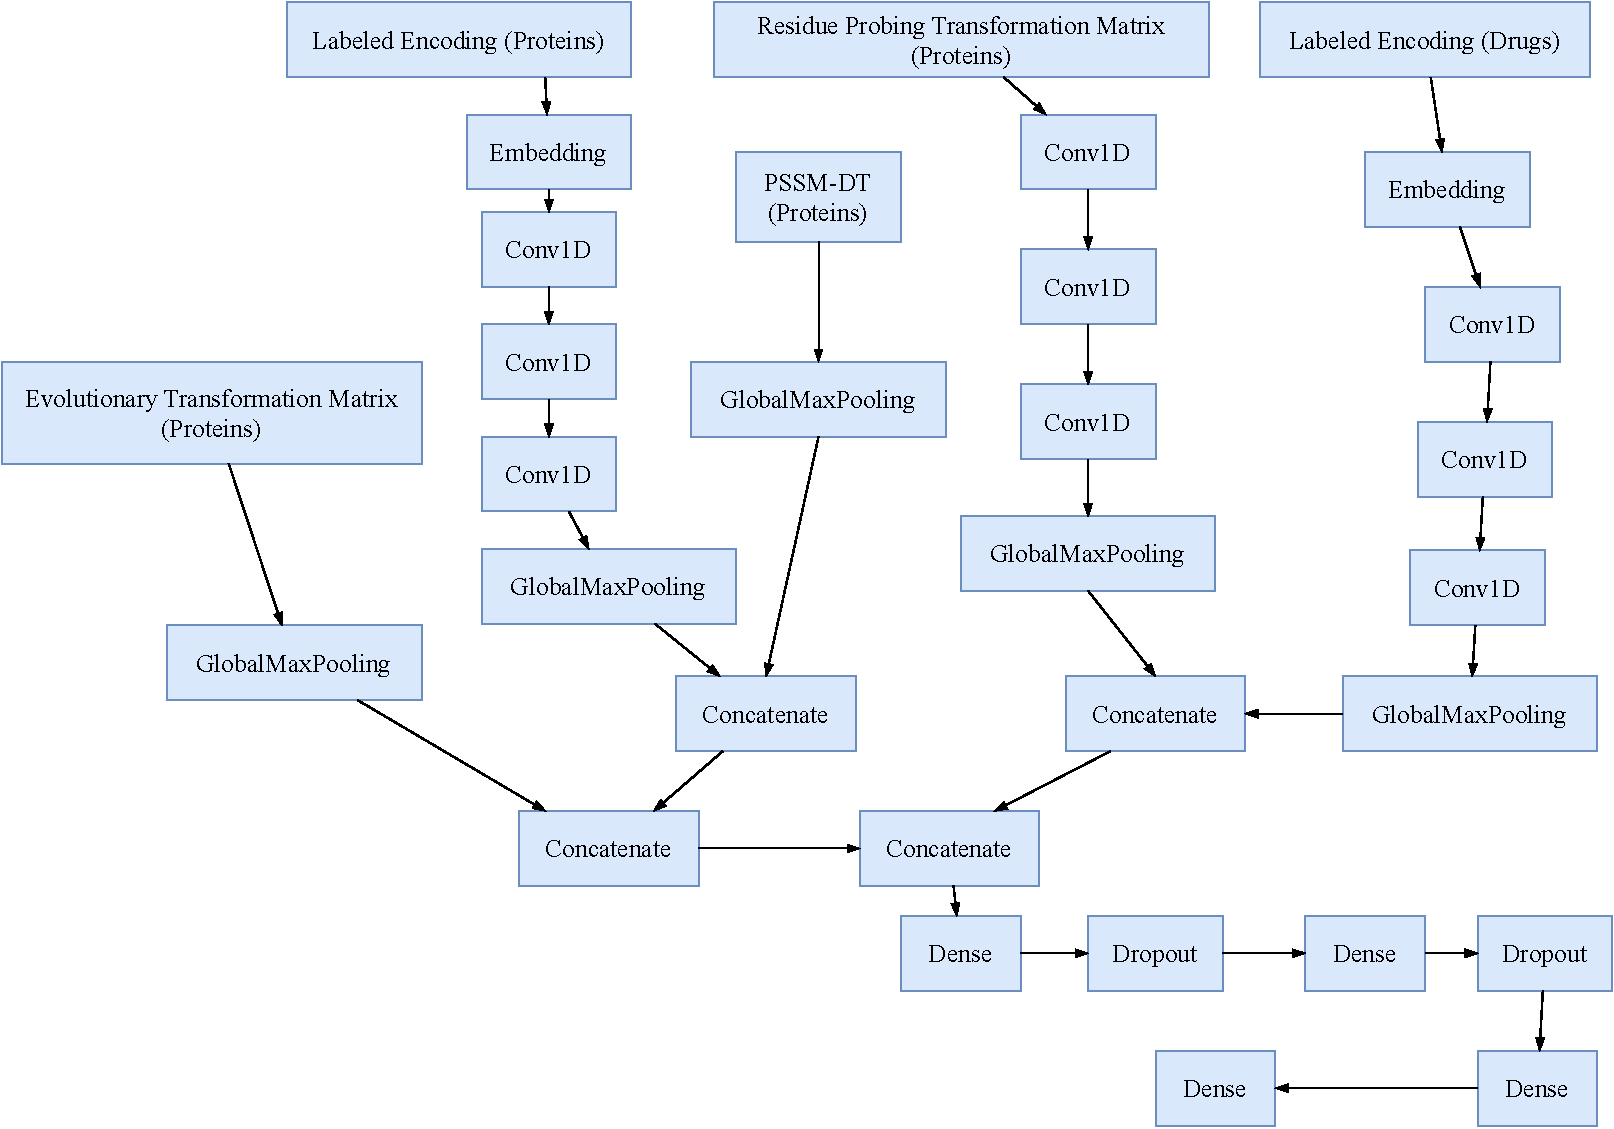
\includegraphics[width=1\linewidth]{mainmatter/3-Methodology/images/DeepDF.pdf}
  \caption{Deep Learning Model to predict Protein-Drug Interaction}
  \label{fig:dlm}
  \end{figure}
  \begin{table}[H]\centering
    \caption{Inputs Used in the Deep Learning Network} 
    \begin{tabular}{|l|l|l|l|}
      \hline 
      S.No. & Input Layer Name & Used Feature Vector & Type \\ \hline
      1 & input\_1 & Label Encodings & Drug \\ \hline
      2 & input\_2 & Label Encodings & Protein \\ \hline
      3 & input\_3 & Evolutionary Distance Transformation Vector& Protein \\ \hline
      4 & input\_4 & PSSM-DT Vector & Protein \\ \hline
      5 & input\_5 & Residue Probing Transformation Vector & Protein \\   \hline 
    \end{tabular} 
    \label{table:inputs}
  \end{table}
  
  \subsection{Components description used from Tensorflow (Keras)}
  \subsubsection{Embedding Layer}
  From figure~\ref{fig:dlm}, the Embedding feature provided by keras for vector representation of both drug fingerprint and protein sequence are utilized. The one-hot encodings of the drugs and protein sequences are inputs to this layer. It turns positive integers (indexes) into dense vectors of fixed size. eg. [[4], [20]] -> [[0.25, 0.1], [0.6, -0.2]].

  \subsubsection{Convolution Neural Network}
  To learn the local patterns in the input vector, we use \acrshort{cnn}. While Dense Layers can learn the global parameters, \acrshort{cnn} is used to understand the local patterns. It does so by increasing the depth layer, which in turn is designed to learn different patterns as shown in Figure ~\ref{fig:cnn}.
  \begin{figure}[H]
    \centering
    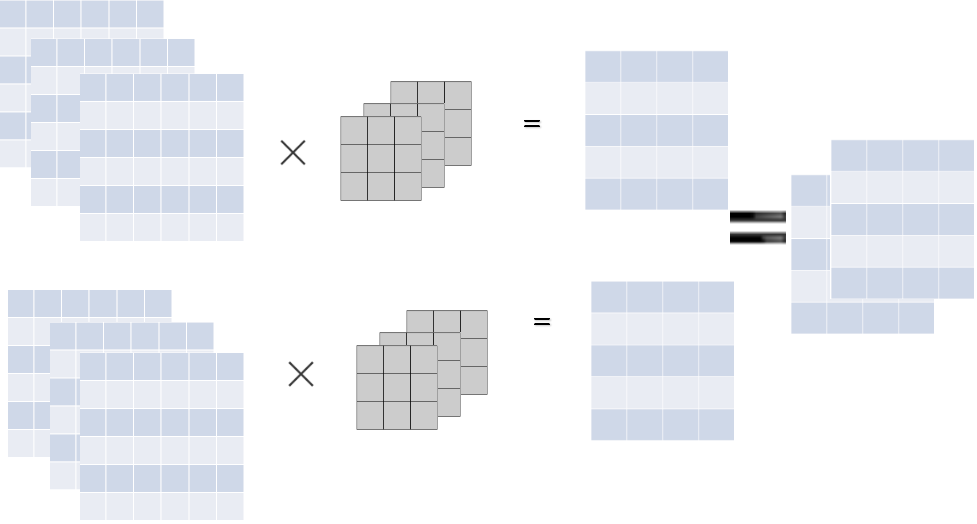
\includegraphics[width=.8\linewidth]{mainmatter/3-Methodology/images/cnn.png}
    \caption{Convolutional Neural Network}
    \label{fig:cnn}
  \end{figure} 

  \begin{figure}
    \centering
    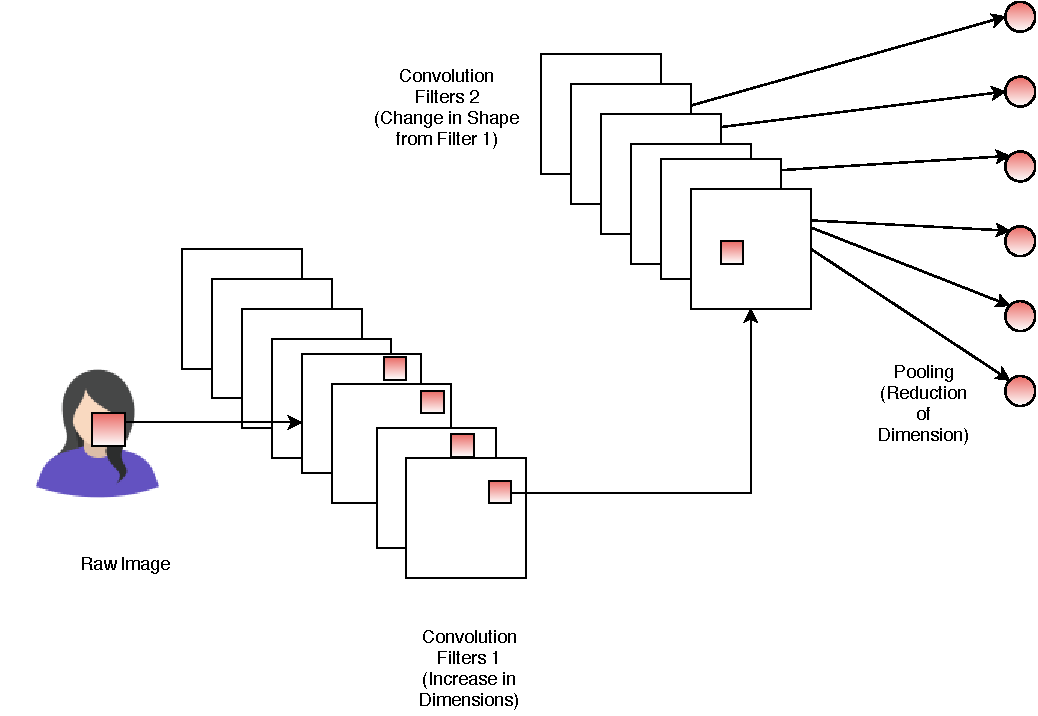
\includegraphics[width=.5\linewidth]{mainmatter/3-Methodology/images/System-Block-CNN-Layer.pdf}
    \caption{Working of CNN Block}
    \label{fig:cnn-2}
  \end{figure}
  
  \subsubsection{Dense Layer}
  Dense Layer is a neural layer which fully connects the input layer to output layer. It can be used to learn the global pattern of the feature data. The representation can be seen from Figure ~\ref{fig:dense}.
  \begin{figure}[ht]
    \centering
    % 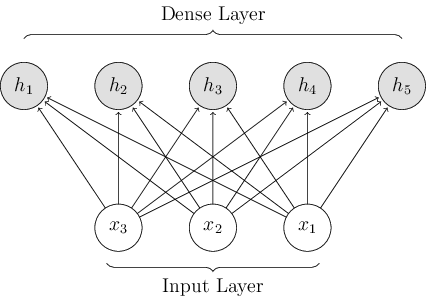
\includegraphics[width=.5\linewidth]{mainmatter/3-Methodology/images/dense.png}
    
  

\begin{tikzpicture}[->,>=stealth',shorten >=1pt,auto,node distance=2.8cm,
    semithick]

      \tikzstyle{every state}=[text=black]
      \node[state]          (A)   {$h_1$};
      \node[state]         (B)  [right of=A] {$h_2$};
      \node[label=above:{Dense Layer},state]         (C) [right of=B] {$h_3$} ;
      \node[state]         (D) [right of=C] {$h_4$};
      \node[state]         (E) [right of=D] {$h_5$};

      \node[state]         (X1) [below of=B] {$x_3$};
      \node[state, label=below:{Input Layer}]         (X2) [right of=X1]       {$x_2$};
      \node[state]         (X3) [right of=X2]       {$x_1$};

      \path (X1) 
      edge              node {} (A)
      edge              node {} (B)
      edge              node {} (C)
      edge              node {} (D)
      edge              node {} (E)
      % edge              node {1,1,R} (C)
      (X2) 
      edge              node {} (A)
      edge              node {} (B)
      edge              node {} (C)
      edge              node {} (D)
      edge              node {} (E)
      % edge              node {0,1,L} (C)
      (X3)
      edge              node {} (A)
      edge              node {} (B)
      edge              node {} (C)
      edge              node {} (D)
      edge              node {} (E);
      % edge [bend left]  node {1,0,R} (E);

\end{tikzpicture}

  
\caption{Dense Layer}
\label{fig:dense}
\end{figure}

  
  \subsubsection{Dropout Layer}
  Our model becomes undesirable when every component of the input layer makes a significant change to the output layer. To reduce the effect of unimportant features the dropout layer was used. Thus the backpropagation network tries to ignore the noise features and minimizes the unrealizable prediction of the learning problem. This can be expressed diagrammatically in Figure ~\ref{fig:dropout}.
  \begin{figure}
    [H] \centering
    \captionsetup{justification=justified}
    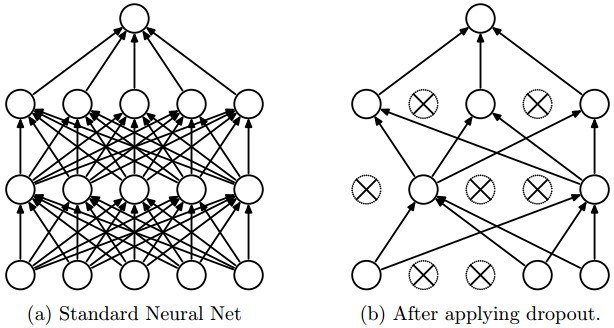
\includegraphics[width=.5\linewidth]{mainmatter/3-Methodology/images/dropout.jpeg}
    \caption[Dropout Layer]{a) Standard neural network whose all the nodes have weights connected to higher nodes and lower nodes. 
    b) Certain nodes belonging to same levels are disconnected. Some weights are also disconnected from other nodes depending on the percentage of dropout applied.}
    \label{fig:dropout}
  
  \end{figure}
  
  \subsubsection{Pooling Layer}
  The Pooling layer is used to downsample the learned parameters from the grid of 3 dimensions returned by Convolution Layer. It gets reduced to 1 dimension by taking the highest values from the window size(corresponding to shape of 1\textsuperscript{st} dimensional element).
  \begin{figure}[H] \centering
    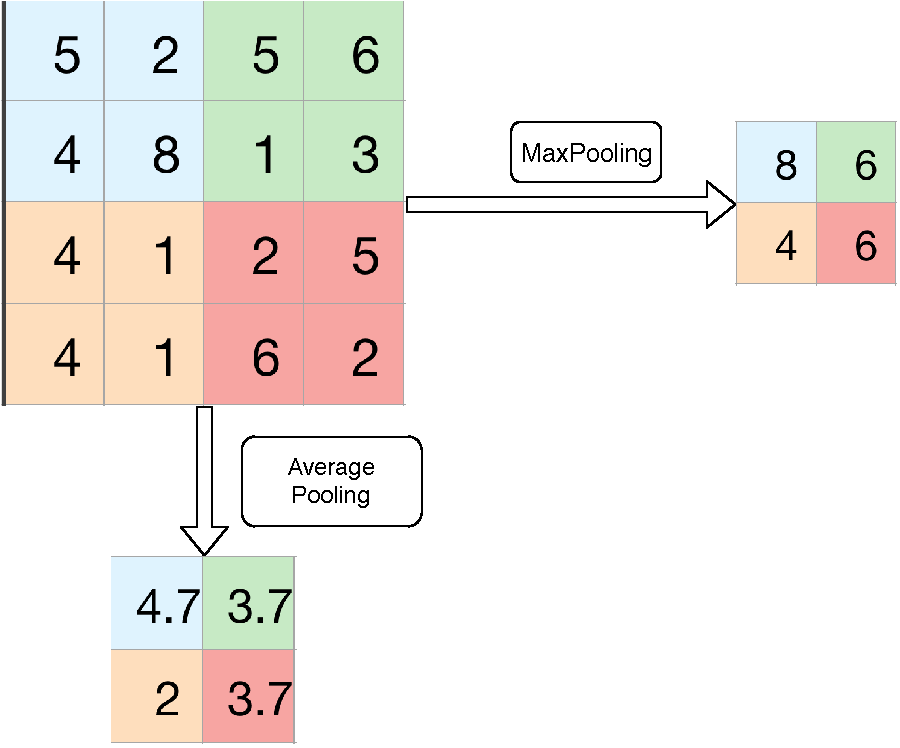
\includegraphics[width=.5\linewidth]{mainmatter/3-Methodology/images/pooling.pdf}
    \caption{Pooling Layer}
    \label{fig:pool_layer}
  \end{figure}
  
  \subsubsection{Concatenation Layer}
  Concatenation Layer as the name implies is used to simply join two vectors so that a feature set comprising of multiple features can be created. Their positional index indicates the feature set being manipulated.
  
  \iffalse
  \subsubsection{LSTM}
  As the \acrfull{rnn} often suffers from vanishing gradient problem~\footnote{Vanishing Gradient:During the training of RNN, the model vectors form a part of a loop and makes an unstable network.}, we use a \acrshort{lstm} Layer to learn the global pattern of the feature sets resulting after concatenation of different stacked layers outputs. The LSTM architecture can be seen in Figure ~\ref{fig:lstm}:
  \begin{figure} 
    [t]
    \centering
    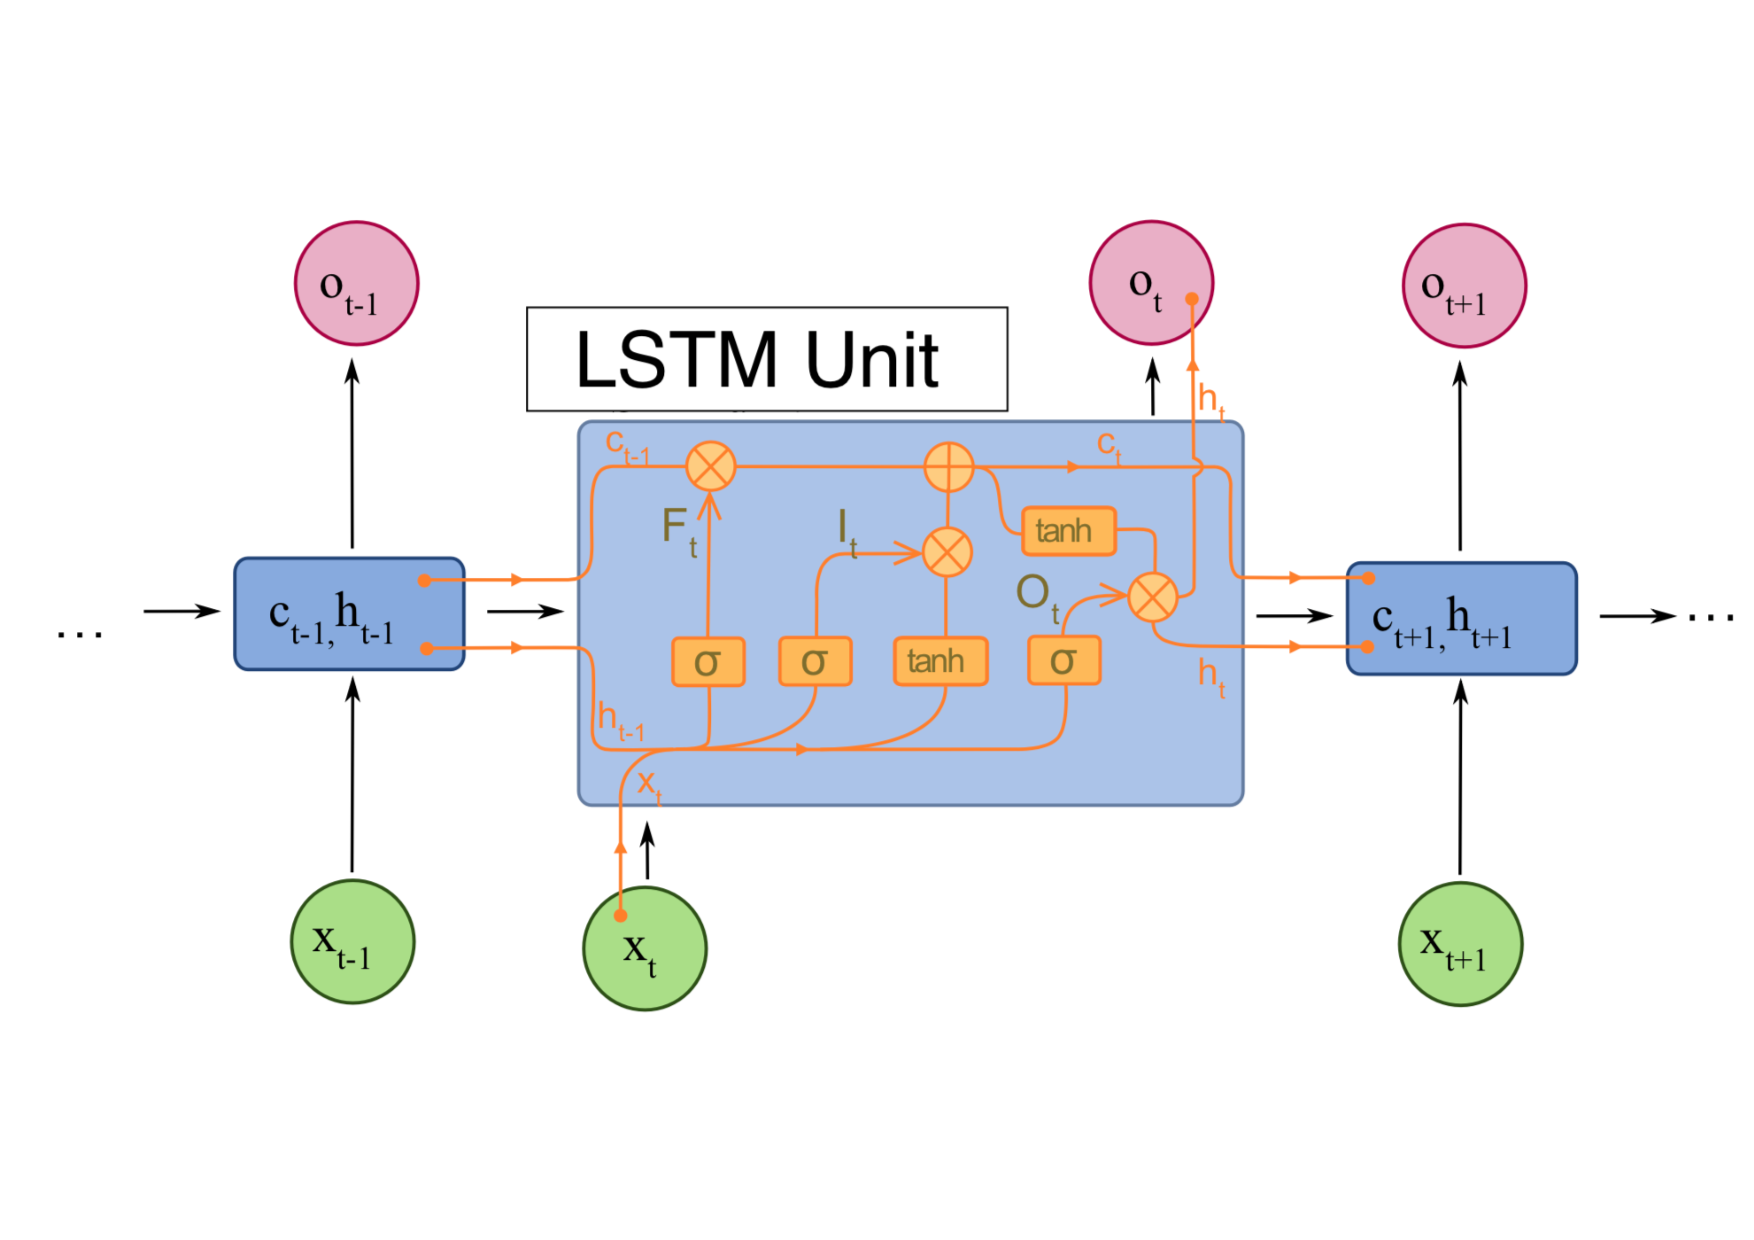
\includegraphics[width=1\linewidth]{mainmatter/3-Methodology/images/LSTM.pdf}
    \caption{Long Short Term Memory}
    \label{fig:lstm}
  \end{figure}
  In Figure~\ref{fig:lstm}, we can see that it contains a forget node, memory node and output node. These three nodes balance the information that needs to be removed, stored for future updates and necessarily fire the output node to make correct prediction.
  \fi